\documentclass[a4paper, oneside, 10pt, draft]{amsart}

\usepackage[utf8]{inputenc}
\usepackage[T1]{fontenc}
\usepackage[english]{babel}
\usepackage[babel=true,kerning=true]{microtype}

\usepackage{amsmath, amssymb}
\usepackage{eucal}
\usepackage{multicol}
\usepackage{enumitem}
\usepackage{mathtools}
\usepackage{standalone}
\usepackage{caption}

\usepackage{stmaryrd}
\usepackage[noend]{algpseudocode}

\usepackage{tikz}
\usetikzlibrary{decorations.markings}
\usetikzlibrary{arrows}
\usetikzlibrary{fit}
\usetikzlibrary{backgrounds}
\usetikzlibrary{positioning}
\usetikzlibrary{decorations.pathmorphing}
\usetikzlibrary{arrows.meta}

\def\osrank{\textsc{\small{osrank}}}
\def\oscoin{\textsc{\small{oscoin}}}
\newcommand{\radicle}{\textsc{\small{Radicle}}}
\def\pagerank{PageRank}
\def\protocol{\mathcal{P}} % TODO: this is now used for projects
\def\netgraph{\mathcal{N}}
\def\accAddrs{\mathcal{A}}
\def\users{\mathcal{U}}
\def\projs{\mathcal{P}}
\def\bal{\mathsf{bal}}
\def\seedset{\Upsilon}

\def\depend{\mathsf{depend}}
\def\undepend{\mathsf{undepend}}

\newcommand{\state}{\mathcal{S}}
\newcommand{\ledger}{\mathcal{L}}
\newcommand{\tuple}[1]{\langle#1\rangle}
\newcommand{\mathsc}[1]{\text{\normalfont\scshape#1}}
\newcommand{\dep}{\xrightharpoondown[e]{d}}
\newcommand{\tx}[2]{\mathsf{#1}\small{\lparen#2\rparen}}

\newcommand{\field}[2]{#1_{\mathsf{#2}}}

\newcommand{\fn}[2]{\mathsf{#1}(#2)}
\newcommand{\prop}[2]{#1.{\mathrm{#2}}}

\newcommand*\eg{e.g.\ }
\newcommand*\ie{i.e.\ }

% No paragraph indentation after section headers.
\makeatletter
\let\@afterindenttrue\@afterindentfalse
\makeatother

\newenvironment{fig}
  {\par\bigskip\noindent\minipage{\linewidth}}
  {\endminipage\par\bigskip}

\newenvironment{epigraph}[2][]
{\leftskip=1cm \def\epigraph@author{#2} \smallskip\itshape}
{\par\vspace{0.5em}\normalfont\hfill---\ \Small\epigraph@author\hspace*{0.2cm}\par\medskip}
\makeatother

\setlist[description]{leftmargin=0.8cm, labelindent=\parindent}
\setlist[itemize]{leftmargin=0.8cm, labelindent=\parindent}
\setlist[enumerate]{leftmargin=0.8cm, labelindent=\parindent}

\setlength{\textwidth}{\paperwidth}
\addtolength{\textwidth}{-4cm}
\setlength{\textheight}{\paperheight}
\addtolength{\textheight}{-4cm}

\calclayout

\begin{document}

\title[open source coin]{open source coin \\ \vspace{0.5em}\Small{trust and sustainability in open source communities} \\ {\tiny Draft 1.0}}
\author{Monadic}
\date{2019}

\begin{abstract}
\small While cryptocurrencies introduced a solution to the problem of digital
scarcity and enumeration, they have failed to create sustainable incentives for
the developers that participate in them.  In this paper we introduce a
cryptocurrency that rewards and provisions open-source software, as well as a
platform for establishing trust and transparency in open source communities.
\end{abstract}

\maketitle

\setlength{\columnsep}{1cm}
\begin{multicols}{2}

\medskip

\section{Background}

\begin{epigraph}{The Open-Source Everything Manifesto}
    \noindent It is in this light that we must recognize that only a restoration of
    open-source culture, and all that enables across the full spectrum of
    open-source possibilities, can allow humanity to harness the distributed
    intelligence of the collective and create the equivalent of heaven on Earth
    --- in other words, a world that works for all.
\end{epigraph}

\subsection{Cryptocurrencies and money}

With the advent of digital scarcity, it became possible to economically
incentivize and remunerate network participants simply and transparently,
without need of a trusted third-party. The introduction of
Bitcoin~\cite{bitcoin}, and later Ethereum~\cite{ethereum}, led to the
proliferation of alternative cryptocurrencies that would primarily compete on
network utility and the monetary policy of assets they provisioned.

If Bitcoin sought to reward network operators for their services validating
transactions, projects such as Zcash and Decred extended this concept to
incentivizing developers and other value producers in order to further stimulate
their respective economies. Despite these experiments, until today, no cryptocurrency
has succeeded in creating sustainable incentives for developers who either
contribute directly to the protocol, or indirectly to the underlying open source
infrastructure.

However, this is one example among the many free and open source software projects
now facing incentivization challenges, a problem that has been
discussed extensively in previous literature~\cite{roads and bridges}.

\subsection{Developer incentives and sustainability}
\label{s:incentives}

To further motivate this work, let us familiarize ourselves with the
conditions in which free and open source software\footnote{In this work, we
shall use the terms \emph{open source software} and \emph{free software} interchangeably,
to mean \emph{software distributed under terms that allow users to run it
for any purpose, as well as change and re-distribute its source code.}}
is developed. Most of the software we use on a daily basis relies on free,
publicly available code. In an increasingly digitized society, free software
projects have become the foundation of digital infrastructure underpinning many
of our societal goods and services.

With the emergence of software hosting sites like GitHub and community sites
like Stack Overflow, open source became the preferred software engineering
paradigm, resulting in numerous high quality projects published in the open,
available for anyone to use. This phenomenon helped
companies reduce lead times and bring products to the market faster, as well as
recruit talent from a new pool of technologists educated on the basis of
free and open source software.

Today, many free software projects start with individuals or small groups
solving a personally, socially, or technologically relevant problem.
Reviewing their motivation for participating in the free software ecosystem,
certain themes emerge: pride in one's work, reputation, learning,
responsibility for something they believe in, and being part of a community.

While most open source software projects start for the reasons above, those
that gain momentum require significant time and financial resources to
maintain. This creates a fundamental problem: an important subset of projects
started in a developer's spare time are becoming critical public
infrastructure. And while some developers find ways to finance their efforts,
most struggle to keep up with community requests during their free time, often
abandoning their projects or burning out under the burden of increasing
responsibility. It is this problem, developing a healthy and sustainable means
of open source maintenance and financing, that we address in this work.

\section{The Oscoin Network}
\label{s:oscoin}

\noindent In this paper, we introduce \oscoin{}, a cryptocurrency protocol
designed to provide a solution to the open source sustainability problem.

\oscoin{} is a public network of distributed computers participating in a
protocol for coming to consensus on a shared transaction ledger.

This ledger is materialized into a global state $\state$ which
contains the canonical registry $\registry$ of all open source
projects participating in the \oscoin{} protocol; a set of accounts
$\accounts$, containing the balances of all currency holders; and
a network graph $\netgraph$, of the relevant relations between
entities in the network, including dependencies between
registered projects and project contributions.

The purpose of this network is to secure a digital currency---\oscoin{}---and
reward the most valued open source projects in the network, without the need
for intermediaries or central control.

\subsection{The Oscoin Blockchain}

To design a safe, open (``permissionless'') currency, shared amongst all network
participants, we propose creating an \oscoin{} blockchain protocol, following
work described by Nakamoto in \cite{bitcoin} and Wood in \cite{ethereum}.

Though the specific choice of the underlying consensus mechanism is not
directly relevant to \oscoin{}, we believe that one which allows open
participation is best for the long term health of the network. Furthermore,
it's important that reliable support for light clients be possible. The only
family of blockchain protocols with these characteristics are the proof-of-work
protocols.

% TODO: you might get some pushback saying the consensus mechanism is 'not relevant'

\begin{figure*}[!ht]
    \par\medskip\noindent\minipage{\linewidth}
    \centering
    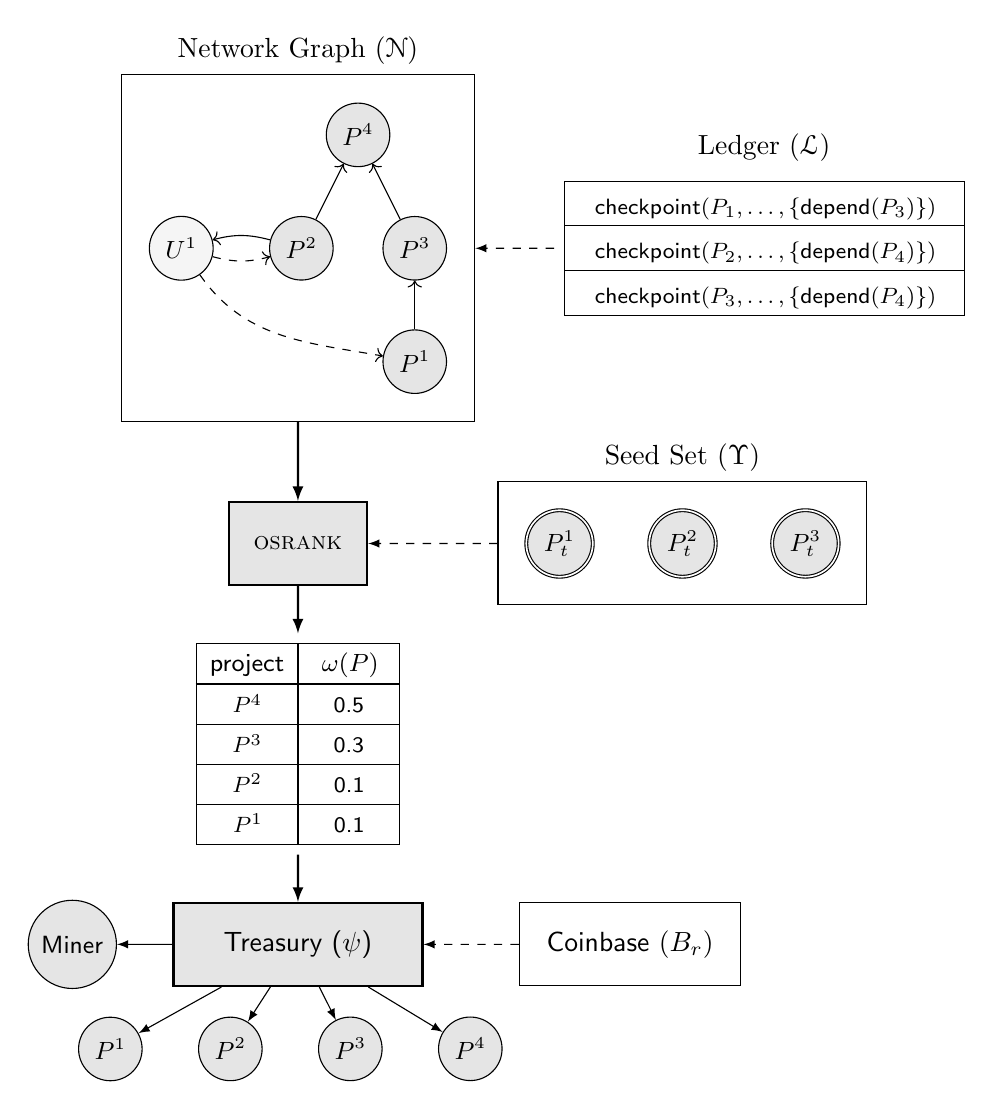
\begin{tikzpicture}[scale=0.96]
    \usetikzlibrary{matrix}

    \tikzset{
        table/.style={
            matrix of nodes,
            row sep=-\pgflinewidth,
            column sep=-\pgflinewidth,
            anchor=center,
            nodes={rectangle, draw=black, text width=7ex, align=center},
            text depth=0.2ex,
            text height=1.6ex,
            nodes in empty cells
        },
        texto/.style={font=\footnotesize\sffamily},
        title/.style={font=\footnotesize\sffamily}
    }
    \tikzset{
        ledger/.style={
            matrix of nodes,
            row sep=-\pgflinewidth,
            column sep=-\pgflinewidth,
            anchor=center,
            nodes={rectangle, draw=black, text width=32ex, align=center},
            text depth=0.2ex,
            text height=2ex,
            nodes in empty cells
        },
        tx/.style={font=\footnotesize\sffamily},
    }
    \tikzset{edge from parent/.style={draw, <-}}

    \tikzstyle{thick-arrow} = [thick, -latex]
    \tikzstyle{proj-seed}   = [draw, double, fill=black!10, circle, minimum height=2em, minimum width=2em, node distance=2em];
    \tikzstyle{proj-s}      = [draw, fill=black!10, circle, minimum height=2em, minimum width=2em, node distance=2em];
    \tikzstyle{user-s}      = [draw, fill=black!4, circle, minimum height=2em, minimum width=2em, node distance=2em];
    \tikzstyle{miner}       = [draw, fill=black!10, circle, minimum height=2em, minimum width=2em, node distance=2em];
    \tikzstyle{proj-group}  = [draw, fill=white, rectangle, minimum height=3em, minimum width=3em, node distance=3em];
    \tikzstyle{process}     = [draw, thick, fill=black!10, rectangle, minimum height=3em, minimum width=5em];
    \tikzstyle{coinbase}    = [draw, fill=white, rectangle, minimum height=3em, minimum width=8em, node distance=10em];
    \tikzstyle{pointer}     = [thin, dashed, -latex];

    %
    % Project dependency graph
    %
    \node[proj-s] (proj-a-4)  [] {\small{$P^4$}}
        child { node[proj-s] (proj-a-2)  [] {\small{$P^2$}} }
        child {
            node[proj-s] (proj-a-3)  [] {\small{$P^3$}}
                child { node[proj-s] (proj-a-1) [] {\small{$P^1$}} }
        };

    \node[user-s] (user-a) [left=of proj-a-2] {\small{$U^1$}};

    \begin{scope}[on background layer]
        \node (netgraph) [proj-group,
            label={Network Graph ($\netgraph$)},
            inner sep=10pt,
            fit=(proj-a-1) (proj-a-2) (proj-a-3) (proj-a-4) (user-a)] {};
    \end{scope}

    %
    % Ledger
    %
    \matrix[ledger, label={Ledger ($\ledger$)}, right=of netgraph] (ledger) {
        |[tx]| $\tx{checkpoint}{P_1, \ldots, \{\depend(P_3)\}}$                       \\
        |[tx]| $\tx{checkpoint}{P_2, \ldots, \{\depend(P_4)\}}$                       \\
        |[tx]| $\tx{checkpoint}{P_3, \ldots, \{\depend(P_4)\}}$                       \\
    };

    %
    % OSRANK
    %
    \node[process] (osrank) [below=of netgraph] {\osrank{}};

    %
    % Seed set projects
    %
    \node[proj-seed] (trusted-1)  [right=2cm of osrank]    {\small{$P^1_t$}};
    \node[proj-seed] (trusted-2)  [right=of trusted-1]     {\small{$P^2_t$}};
    \node[proj-seed] (trusted-3)  [right=of trusted-2]     {\small{$P^3_t$}};

    \begin{scope}[on background layer]
        \node [proj-group, label={Seed Set ($\seedset$)},
            inner sep=10pt, fit=(trusted-1) (trusted-2) (trusted-3)] {}
                edge [pointer] (osrank.east);
    \end{scope}

    \matrix[table, below=0.6cm of osrank] (weights) {
        |[title]| \small{project} & |[title]| \small{$\omega(P)$} \\
        \hline
        |[texto]| $P^4$            & |[texto]| 0.5             \\
        |[texto]| $P^3$            & |[texto]| 0.3             \\
        |[texto]| $P^2$            & |[texto]| 0.1             \\
        |[texto]| $P^1$            & |[texto]| 0.1             \\
    };

    %
    % Distribution
    %
    \node[process, minimum width=9em] (distribution) [below=0.6cm of weights] {\textsf{Treasury ($\psi$)}};

    % Coinbase
    \node[coinbase, right of=distribution, node distance=12em] {\textsf{Coinbase} ($B_r$)} edge [pointer] (distribution.east);

    %
    % Projects receiving oscoin
    %
    \node[proj-s] (proj-b-1)  [below left=of distribution]    {\small{$P^1$}};
    \node[proj-s] (proj-b-2)  [right=of proj-b-1]             {\small{$P^2$}};
    \node[proj-s] (proj-b-3)  [right=of proj-b-2]             {\small{$P^3$}};
    \node[proj-s] (proj-b-4)  [right=of proj-b-3]             {\small{$P^4$}};

    % Miner
    \node[miner]  (miner)     [left=of distribution]          {\small{\textsf{Miner}}};

    \begin{scope}[on background layer]
        \draw[thick-arrow] (netgraph.south)              to    (osrank.north);
        \draw[thick-arrow] (osrank.south)                to    (weights.north);
        \draw[thick-arrow] (weights.south)               to    (distribution.north);
        \draw[-latex,dashed] (ledger.west)               to    (netgraph.east);

        % Distribution arrows
        \draw[-latex] (distribution)              to    (proj-b-1);
        \draw[-latex] (distribution)              to    (proj-b-2);
        \draw[-latex] (distribution)              to    (proj-b-3);
        \draw[-latex] (distribution)              to    (proj-b-4);
        \draw[-latex] (distribution)              to    (miner);

        % Owner arrows
        \draw[->,dashed] (user-a) to[out=-15,in=-165] (proj-a-2);
        \draw[->] (proj-a-2) to[out=165,in=15] (user-a);
        \draw[->,dashed] (user-a) to[out=-55,in=170] (proj-a-1);
    \end{scope}
\end{tikzpicture}

    \caption{The Oscoin Treasury System\label{f:treasury}}
    \endminipage\par\medskip
\end{figure*}

\subsection{The Oscoin Treasury}
\label{s:treasury}

The treasury subsystem (Figure \ref{f:treasury}) is designed to continuously
rank projects on the network based on relative importance and reward them with
\oscoin{}.

\subsubsection{Overview}

\begin{itemize}
    \item Maintainers and contributors collaborate around software projects
        registered on the network.
    \item Maintainers merge contributions and synchronize their project state
        with the ledger, which includes per-project dependency information and
        contribution metadata (\S\ref{s:checkpointing}).
    \item Every $\epoch$ blocks, the \osrank{} of each project is calculated
        (\S\ref{s:osrank}).
    \item A reward in \oscoin{} is derived from each project's \osrank{},
        and distributed to \emph{projects and contributors} via smart
        contracts (\S\ref{s:smart-contracts}).
\end{itemize}

\medskip

\noindent Each block, the protocol is allowed to mint a certain amount $B_r$ of \oscoin{}
(the ``block reward''), as part of what we call the \emph{coinbase}
transaction. These coins are allocated to two distinct groups: network
operators (``miners''), formally $\miners$, and open source projects ($\projs$)
through the treasury system.

The key question we must answer, is what share of $B_r$ is distributed to
individual projects and contributors in the network.  The goal is to choose
a distribution mechanism that rewards projects in proportion to their relative
importance within the network.

For this, we leverage the \oscoin{} network graph $\netgraph$ (Section
\ref{s:netgraph}), which maps flows of value between projects and contributors,
and assigns a weight to each.

\subsubsection{Algorithm} Let $t$ be the total amount of \oscoin{} distributed
to $n$ projects every epoch $\epoch$. The amount $t_P$ distributed to a given
project $P$ over $\epoch$ is a function of its \osrank{} weight $\omega(P)$,
which rewards higher ranking projects with more \oscoin{}. We describe this
\emph{payment function} as
\[
    \psi(t, \omega(P)) \to t_P
\]
To prevent trivial Sybil attacks, the payment function takes
into account a minimum threshold for $\omega(P)$ under which a project does not
receive funds. Rewards can be further equalized by adjusting $\psi$ to
compress or expand the reward range.

% TODO: equalized perhaps not the right word choice. What does 'equal' mean in this
% context?

In this model, it is the responsibility of maintainers to choose project
dependencies accurately and to keep their stated dependencies up to date, since
dependence on a project is a signal of trust and a vote cast to receive funds.
For projects highly-weighted within the graph, the importance of this signal is amplified.

At scale, this mechanism has the potential to solve many of the issues with
open source monetization and sustainability. Projects can receive
income in the form of \oscoin{}, while licensing their work as free and
open source software (FOSS). Such continuous algorithmic funding moves
away from current ``transactional'' models---which require open source projects
to change the way they work, re-license, setup a business---to a new model,
which aligns with the motivations that lead to the success of the open source
movement (\S \ref{s:incentives}).

% TODO: the appositive in the middle of this sentence makes it difficult to read and
% causes the reader to context switch. I'd recommend talking about the current transactional
% model and then continuous funding, not breaking up the latter.
\section{Osrank}
\label{s:osrank}

\def\Graph{\mathsf{Graph}}
\def\proj{\mathsf{proj}}
\def\user{\mathsf{user}}
\def\dep{\mathsf{dep}}
\def\own{\mathsf{own}}
\def\coown{\mathsf{own}^\circ}
\def\contrib{\mathsf{contrib}}
\def\cocontrib{\mathsf{contrib}^\circ}

Since one of the fundamental mechanisms of \oscoin{} is to distribute a portion
of newly minted tokens to high-value projects on the network, the protocol needs
to reach consensus on which projects are ``high value''. To choose which
projects receive compensation, and in which proportions, the network uses
\osrank{}, which is a modification of the well-know \pagerank{}
algorithm~\cite{pagerank} applied to the graph of relationships between projects
on the network, and in particular \emph{dependencies} between projects. The
output of the algorithm is a score $\omega(P)$ associated to each project
$P$.

\subsection{Rationale}

While it may be clear that value is being produced by a system as a whole, it is
often unclear how much value particular subsystems are
contributing. Furthermore, subsystems have inherently differing capacities to
transform value into revenue: subsystems at the boundaries with other domains
are at an advantage, even though they may (transitively) derive much of their
value from other subsystems. This disbalance in value flows in and out of
subsystems is detrimental to the system as a whole.

Thankfully, human activity does not happen in a void\footnote{Space
  exploration will be addressed in a subsequent paper.}: be it
knowledge work, content/media creation, financial activity, etc.,
entities interact with one another in meaningful ways that are highly
influenced by the relative value each entity has with respect to the
system as a whole. Crucially, during this activity, a trail of
\emph{artefacts} (hypermedia links, contracts, transactions,
dependencies, pull-requests etc.) is produced; concrete manifestations
of the relationships between the various entities.

The basic insight of \pagerank{} and similar metrics, is that by
stochastic simulation of meaningful activity traces of system agents,
producing trails of artefacts consistent with observations, one can
learn about the value flows between subsystems, and hence approximate
the underlying value distribution. In the case of \pagerank{} one
simulates a human searching for high-relevance data over the internet,
following a chain of links. A sophisticated algorithm would use as
many heuristics as possible for choosing the next link to follow (as a
real human would), \eg{} evaluating the relevance of the link-text. If
computational resources are scarce, the crudest algorithm simply picks
the next link at random, and this is what produces the classic
\pagerank{} formula which has seen so much success at ranking web
pages.

The artefacts related to OSS development which are captured on the \oscoin{}
ledger are:
\begin{itemize}
  \item Ownership of a project by a user,
  \item Dependencies between projects,
  \item Contributions of code from users to projects.
\end{itemize}

\begin{center}
\begin{tikzpicture}[vertex/.style={draw,circle}, arr/.style={draw,thick,->}]
  \node[vertex] (p) at (2,0)  {\small $\proj$};
  \node[vertex] (u) at (-2,0) {\small $\user$};

  \draw[arr,looseness=9] (p) to[out=95,in=25] node[above] {\small $\dep \ (4/7)$} (p);
  \draw[arr] (p) to[out=165,in=15] node[above]   {\small $\own \ (2/7)$} (u);
  \draw[arr] (u) to[out=55,in=125] node[above]   {\small $\coown \ (3/5)$} (p);
  \draw[arr] (p) to[out=195,in=-15] node[below]  {\small $\contrib \ (1/7)$} (u);
  \draw[arr] (u) to[out=-55,in=-125] node[below] {\small $\cocontrib \ (2/5)$} (p);
\end{tikzpicture}
\captionof{figure}{\small Entity relations in open source software development. \label{fig:G}}
\end{center}

We summarise this these interactions with a weighted directed graph $G$
(Figure~\ref{fig:G}), the weights corresponding to the relative importance of
the edge, tweaked by our own judgement and informed by simulations we have
run.

% TODO: include simulations description and results here.

The weights on all edges outgoing from a vertex sum to $1$.

Note that some of the edges are biderectional, but each direction gets
it's own weight. For example both $\contrib$ and $\cocontrib$ point to
the same artefact: a contribution of code from a user to a
project. The edge $\contrib$ represents the statement \emph{``the user
  is valuable to the project''}. The edge $\cocontrib$ going in the
opposite direction represents the statement \emph{``the project is
  valuable to the user''}; the rationale for this less obvious flow is
that users are unlikely to invest time contributing to a project they
don't find useful.

% TODO: include similations data.

The \oscoin{} network proposes to record these artefacts as
transactions in a blockchain, so that one may unambiguously rebuild
(and reach consensus on) a finite directed graph $\netgraph$ over $G$
(\ie{} in the slice category $\Graph/G$). We'll refer to $\netgraph$
as the \emph{network graph}.

This in turn allows global value scores to be assigned to entities
according to a specific stochastic process simulating \emph{random
  walks}, that is, activity traces in $\netgraph$ with sampling
probabilities taken from $G$. For example: a contributor decides to
work on a high value project (probably at the border), contributes a
PR, in so doing adds a dependency to another project, which imports a
bug from upstream. The contributor therefore switches to fixing said
bug in the dependency, etc. Much like a simulation of a human
searching for information by clicking through links, this simulated
contributor activity informs us on the value flows between subsystems
in OSS development.

This score, which we call \osrank{}, is used to weight the
distribution of newly minted tokens to high value entities, thus
compensating entities which bring value to the ecosystem.

\subsection{Definition}

More specifically we use the following Monte Carlo-based algorithm: for each
project on the network, $R$ random walks are performed which start at that
node. To decide which next vertex to visit during a random walk, first a type of
outgoing edge is decided by sampling outgoing edges according to the weights in
$G$. The next choice is the specific to the edge:

\begin{itemize}
\item In the cases of $\dep$, $\own$, all vertices are equiprobable.
\item In the cases of $\coown$ and $\cocontrib$ the projects to choose from are
  weighted according to the number of contributions of the owner/user to these
  projects,
\item In the case of $\contrib$, the users are weighted by the number of
  contributions they have made to $P$.
\end{itemize}

At each step the walk might terminate with probability $1 - \epsilon$, (here
$\epsilon$ is the \emph{damping factor}, $0 < \epsilon < 1$). This produces a
set $W$ of walks. The \osrank{} for a project $x$ is then:
\[
  \omega(x) = \frac{W_x \epsilon}{n R}
\]
where $W_x$ is the number of visits of $x$, over all walks, that is:
\[
W_x = \sum_{w \in W} v(w,x)
\]
where $v(w,x)$ is the number of times path $w$ visits the vertex $x$.

\subsection{Fake ecosystems}

The main problem to avoid is compensating fake ecosystems, that is,
project structures and relationships which have been setup in the
network graph for the sole purpose of gaming the \osrank{} algorithm.

For this we propose running \osrank{} in two distinct phases:
\begin{itemize}
\item In the first phase, a seed set $S$ is used as the for the
  beginning of all walks. Specifically, a random walk always starts at
  a vertex in $S$. Otherwise the process remains the same. The scores
  obtained are biased towards interactions with the seed set, but they
  are not used directly by the compensation mechanism. Instead a
  threashold $t$ is used to determine the legitimacy of entities: any
  entity falling below this threshold is not considered for the next
  phase. One obtains a subgraph of the network graph $\netgraph_t$.
\item In the seconds phase, the algorithm is ran on the subgraph
  $\netgraph_t$ as usual, with no seed set. The output of the second
  phase is the \osrank{}.
\end{itemize}

% TODO: remove the term governance.
We propose that the seed set be maintained by an on-chain governance
system, aiming to choose high-value user-facing projects,
e.g. Firefox, Debian, VLC, etc. Care must be taken to ensure the seed
set is large enough to touch most legitimate projects on the network.

\subsection{Implementation}

There are several options for making sure the computation of \osrank{}
will not be prohibitively expensive for operators to run.

\begin{itemize}
\item \emph{Incremental Monte Carlo.} An incremental algorithm is used
  so that \osrank{} values may be updated as the network graph
  evolves. Instead of computing \osrank{} from scratch, we rely on the
  fact that only a small percentage of the nodes and edges of the
  network graph are added or removed from one calculation to the next
  (confirmed empirically on the datasets of major code-hosting
  platforms). Therefore most of the random walks that were performed
  in the previous calculation remain valid in the updated graph. For
  example if only a single dependency $x \to y$ has been added, then a
  walk is invalid only if passes through $x$, for it may have chosen
  to follow this new dependency.

  In practice the operators of the network cache the set of random
  walks from the previous calculation, and update this set by removing
  invalid walks and replacing them with new ones. Details on such an
  incremental algorithm used in the case of \pagerank{} can be found
  in \cite{incr pagerank}.

  Since all the computations must be deterministic, the walks are not
  truly random. Rather, they must use a built-in pseudo-random number
  generator to generate the random walks. The seed for generating
  random walks is fixed in the genesis block.

  % TODO: Add details on RNG

\item \emph{Long epoch.} In this scenario payouts according to
  \osrank{} are only made infrequently, say with a duration of $d$
  between \emph{payout} blocks (e.g.\ once every month). In this case
  abusers might modify network structures of several projects in
  anticipation of the payout block. To mitigate this, some edges are
  weighted by the amount of time it has existed in the last epoch. For
  example, if a dependency is added a day before the payout block,
  then it only has a wight proportional to $1/d$.
\end{itemize}

\section{The Oscoin Ledger}
\label{s:ledger}

The \oscoin{} ledger, formally $\ledger$, is the ordered set of all
transactions agreed upon by the network. The ledger can be updated by submitting
a valid transaction to the network. Transactions operate on the current state
$\state$ of the ledger, which is a materialized view of all processed transactions.

The transactions available on the ledger are described in this section, as well
as how they affect the state $\state$.

\subsection{Supply}

The supply of \oscoin{} is subject to an increase $B_r > 0$ carried out by the
protocol every epoch, following a fixed supply curve. This ensures a continuous
flow of \oscoin{} into the treasury (Section \ref{s:treasury}), to reward work
in the network.

\subsection{Accounts}
\label{s:accounts}

Currency (\oscoin{}) is held in \emph{accounts} which can be unlocked by the
signature of the account holder. Accounts have addresses which are used to send
and receive \oscoin{}. This model follows the design of Ethereum \cite{ethereum}
rather than Bitcoin's UTXO model \cite{bitcoin}.

Accounts are created by sending \oscoin{} to them (Section \ref{s:sending}),
and are removed from the ledger when their balance reaches zero. The set of all
accounts is known as $\mathcal{A}$.

The account balance $A_b$ of an account $A$ is held in the state $\state$, and
can be accessed with the account address $A_a$. Formally, $\state(A_a) \to A_b$.

\subsection{Projects}
\label{s:projects}

A project $P$ is a tuple:
\[
    P = \tuple{P_a, P_h, P_s}
\]
where $P_{a}$ is the project's address and unique identifier, $P_h$ is
the project's current hash and $P_s$ is the canonical project source
URL.

% TODO: Project address is not an integer
The project address, an integer, is used to identify the project, as
well as to send \oscoin{} to it. Each project has an account balance
identified by project address. The project hash is a digest of the
project's source code at the time it is entered in the
ledger. Finally, the project URL is there for convenience, as a means
to fetch the source code.  It must be noted that the source code
retrieved from $P_s$ must always hash to $P_h$, otherwise the project
is considered invalid.

\subsubsection{Registration and ownership} Projects need to be
registered on the ledger before they can participate in the
network. This can be done with the
\[
    \tx{register}{P_a, P_s}
\]
transaction, signed by a key $k_1$ which must be used when updating the project
at a later time. The transaction is valid as long as the address $P_a$ isn't
already in use, and $P_s$ is a valid URL.

On successful execution, the transaction locks a small amount of \oscoin{} from
the account associated with $k_1$. This helps ensures that abandonned projects
don't clutter the ledger.  Once executed, the project is instantiated to $P =
\tuple{P_a, P_h, P_s}$ with $P_h = \varnothing$.

The project $P$'s current key set $P_K$ is $\{k_1\}$. This can be extended
with:
\[
    \tx{addkey}{k}
\]
where $k$ is a valid key not present in $P_K$. Keys can also be removed, with:
\[
    \tx{removekey}{k}
\]
where $k$ is a key present in the $P_K$.
When a project is no longer in use, it is possible to unregister it from the
ledger with
\[
    \tx{unregister}{P_a},
\]
which must be signed by an owner ($k_1$ in the above example).
Execution of this transaction returns the registration deposit to the account
associated with the registration key.

Projects registered on the ledger can be retrieved from the state $\state$ by
using the project address, formally: $\state(P_a) \to P$.

\subsubsection{Checkpointing} \label{s:checkpointing} Any project in active
development will see its source code change regularly. This means the project
hash $P_h$ will quickly become out of sync with the project's latest state and
will need updating. This is done via the
\[
    \tx{checkpoint}{P_a, P_{h'}, P_{s'}, C^*, D^*}
\]
% TODO: what is the use of s?
transaction, where $P_{h'}$ is the new project hash, $P_{s'}$ is the URL to
retrieve the source code from, $C^*$ is a hash-linked-list of
\emph{contributions}, and $D^*$ is a list of \emph{dependency updates}.

Contributions are tuples:
\[
   \tuple{\field{C}{prev}, \field{C}{commit}, \field{C}{author}, \field{C}{signoff}}
\]
where:
\begin{itemize}
\item $\field{C}{prev}$ is the hash of the previous contribution, or
  $\varnothing$ if this is the first contribution to the whole
  project. Note that $C^*$'s first item must be linked to the last
  contribution in the project's \emph{previous} checkpoint, such that no
  gaps between contributions exist.
\item $\field{C}{commit}$ is the hash of the corresponding commit,
\item $\field{C}{author}$ is the author of the contribution,
\item $\field{C}{sig}$ is the author's signature of $\field{C}{commit}$.
\item $\field{C}{signoff}$ is the \emph{signoff key}, which must be $\in P_K$.
\end{itemize}
A contribution must be signed by the signoff user. This signals the
the contribution has been reviewed/verified by this maintainer. The
checkpoint as a whole must also be signed by a key in the project key set.

Because all changes to a project's source code are signalled by checkpoints, it
is possible to reconstruct a full hash-linked list of contributions for the
entire project. When cross-referenced with the project's repository, this gives
a full historical breakdown of who authored which code, and which project
maintainer signed it off.  This makes the project history auditable and
tamper-proof, as well as providing valuable information to the \osrank{}
algorithm. Note that only the contribution \emph{metadata} is stored on-chain.

\label{s:dependencies}
Conceptually, a project $P$ depends on a project $P'$ if it is an
``input'' to $P$ in some way: $P$ references $P'$ or parts of
$P'$ in its source code, or $P'$ is a build/test dependency.
For example if a project used the purely functional package
manager \emph{Nix} \cite{nix}, then the dependencies declared on
\oscoin{} should probably map one to one with the Nix
dependencies. Dependencies are an important input to the \osrank{}
metric.

The dependencies updates list $D^*$ is a list of \emph{dependency
  updates}, which are one of
\[
    \depend(P'_a, n) \quad \text{or} \quad \undepend(P'_a, n)
\]
which refers to the $n$th checkpoint of a project $P'$ ($0$-indexed
from the first checkpoint). The $\depend$ update adds a new dependency
while the $\undepend$ update removes a dependency. The updates are
processed in order with $\depend$ only being valid if it adds a
dependency that the project doesn't already have and $\undepend$
only being valid for current dependencies. The checkpoint is invalid
if the update list contains duplicates.

As a project owner, adding a dependency signals a variety of things
(partly dependent of the nature of the project):
\begin{itemize}
\item they have verified that $P$ indeed depends on this specific
  version of $P'$,
\item that $P'$ is suitable as a dependency for $P$, \eg{} if $P$ has
  very high security requirements, that $P'$ fulfils these.
\end{itemize}

\def\posnat{\mathbb{N}_{\geq 1}}

\subsection{Sending \oscoin{}}
\label{s:sending}

Each user is associated with an \oscoin{} balance. Projects are associated with
two accounts, the first is the \emph{project account} and is controlled by the
owners. The second is the \emph{project fund}, and is controlled by smart
contracts (see \S \ref{s:smart-contracts}). The set of \emph{balance addresses}
is the coproduct of the set of user keys and the set of project addresses:
\[
    \accAddrs = \users + \projs.
\]

Each address is associated to a balance:
\[
    \bal(a) \in \posnat \mid a \in \accAddrs.
\]

Transfers to and from balances are performed by the
\[
    \tx{transfer}{x,y,n} \mid x,y \in \accAddrs, n \in \posnat
\]
transaction. If $x \in \users$ then the transaction is valid if signed by
$x$. If $x \in \projs$ then the transaction is valid if it is signed by a
project owner. In any case, for the transaction to be valid $\bal(x) \geq n$
must hold, and after the transaction $x$'s balance is decremented by $n$ and
$y$'s is incremented by $n$.


\section{Smart contracts}

The \oscoin{} blockchain uses smart contracts as a way to distribute funds that
a project has received. These smart contracts are added with special
transactions which modify the behaviour of a project. For example to control how
funds from the core mechanism payouts are distributed, a project could use the
following code:

\begin{lstlisting}
(fn [proj reward]
  (let [cs    (lookup :contributors p)
        n     (length cs)
        share (div reward n)]
    (map (fn [c]
           [:transfer (lookup :address p) (lookup :address c) share])
         cs)))
\end{lstlisting}

This is a function which is invoked every time project $P$ gets a network
reward. The argument \texttt{proj} is a dictionary containing the project
metadata, while \texttt{reward} is a natural number representing the amount of
oscoin that was awarded to the project. The function must return a list
transactions.

% TODO: add code examples.

\section{Applications and future work}

\oscoin{} as a platform has the potential to enable novel applications for
software communities. In comparison to a general purpose computer like
Ethereum, \oscoin{} provides primitives focused towards code collaboration
(Section \ref{s:ledger}) and enables developers to combine them in flexible ways.

While it’s hard to describe all the possible ways \oscoin{} might be used, we
believe the following categories of applications can benefit from \oscoin{}’s
architecture.

\subsection{Governance and collective decision making}

In the first category, we believe that developers could leverage \oscoin{}’s
network graph ($\netgraph$) in order to make collective decision through smart
contracts.  Developers will have the ability to design smart contracts that
leverage the network graph in order to align interests between all network
participants of an open source project and incentivize further participation.
In addition, smart contracts can be used within these organizations in order to
coordinate around contentious decisions, using a diverse set of decision making
modules.

\subsection{Trust minimization for software development processes}
The second category of applications leverages the availability of contribution
histories on chain, in order to design new software development processes that
minimize trust between network participants.

Rather than relying on the weak trust model of existing centralized hosting
providers, oscoin can be used to create powerful continuous integration
pipelines that use cryptography to ensure that every commit can be trusted.

This category of applications is particularly relevant to high-assurance
software such as cryptocurrencies.

\subsection{Incentivization}
The third category of applications we forsee is the one related with
developer incentives. This might include applications that a) expose paid work
within the oscoin network, b) describe and enforce service level agreements
between projects and their dependencies, or d) re-imagine crowd-funding
applications such as Patreon, taking advantage of digital money and collectibles.

\subsection{DAOs}
% TODO: DAOs

% TODO: Conclusion / future work


\end{multicols}

% TODO: fix formatting in refs, or use bibtex or something.
\begin{thebibliography}{9}

\bibitem{roads and bridges} Eghbal, Nadia. Roads and Bridges. The Unseen labor
  behind our digital infrastructure. July 2016.

\bibitem{pagerank} Brin, S.; Page, L. (1998). The anatomy of a
  large-scale hypertextual Web search engine (PDF). \emph{Computer Networks
  and ISDN Systems.} 30: 107–117.

\bibitem{incr pagerank} Bahmani, Bahman and Chowdhury, Abdur and Goel,
  Ashish. Fast Incremental and Personalized PageRank. Proc. VLDB
  Endow. December 2010.

\bibitem{nix} Dolstra, E., de Jonge, M. and Visser, E. Nix: A Safe and
  Policy-Free System for Software Deployment. In Damon, L. (Ed.), 18th Large
  Installation System Administration Conference (LISA '04), pages 79–92, Atlanta,
  Georgia, USA. USENIX, November 2004.

\bibitem{bitcoin} Nakamoto, Satoshi. Bitcoin: A Peer-to-Peer Electronic Cash
  System. May 2009

\bibitem{ethereum} Wood, Gavin. Ethereum: A Secure Decentralised Generalised
  Transaction Ledger. December 2018

\end{thebibliography}

\end{document}
